\chapter{Introduction}
\section{Aim and scope of the research}

The current research can be situated at the crossroads of several sub-fields of linguistics: historical linguistics, areal linguistics and \isi{language contact}, as well as dialectology, all informed by \isi{linguistic typology} and framed within structuralist linguistics (see the second chapter for a more precise statement of the theoretical framework).  More precisely, I wish to study the variation in a specific language group, namely the \textsc{North-Eastern Neo-Aramaic} dialects (=\ili{NENA}, belonging to the \ili{Semitic} language family -- see below for further information), examine the diachronic origin of the attested variation, and relate it to \isi{language contact} with neighbouring languages as well as to general typological tendencies.

The \ili{NENA} group is well suited for such a study for several reasons: First and foremost, it offers a rich variety of dialects, of  which many have in recent years been described, thus providing a firm empirical underpinning to the research.\footnote{I use the traditional term \enquote{dialects}, but it should be borne in mind not all these dialects are mutually intelligible, and they may represent varieties of different \enquote{languages} of the \ili{NENA} group.} Secondly, as these dialects span a large geographic area, covering north Iraq, south-east Turkey and west Iran, they have been in contact with different languages and language families (mostly \ili{Turkish}, \ili{Azeri}, Kurdish, \ili{Persian} and \ili{Arabic}), thus providing the possibility to study the effects of differing \isi{language contact} situations. Thirdly, previous strata of Aramaic are known and documented, giving the possibility to add diachronic depth to the study. In short, the \ili{NENA} languages are in a unique position, in which the linguistic community have access to both historical strata and to \isi{language contact} data. Thus, they provide  a \enquote{laboratory} setting in which it may be possible to disentangle the role of \enquote{pure} language-internal change from changes originating in particular \isi{language contact} situations. My conclusions, I hope, could inform linguists looking at linguistic change in languages which do not have this wealth of information.

As I am working in a \isi{language contact} framework, I am mainly interested  in overt patterns, or -- more technically, constructions -- prone to replication from one language to another. Thus, a specific construction (with a given function)  is defined in terms of the linear (syntagmatic) ordering of its elements, together with the morphological cues present on each element.
In contrast to some formal approaches, I am less interested in covert elements, or the hierarchical (syntactic) relations between the elements. As such, the research is focused on the \enquote{surface} manifestation of linguistic content. 

To establish the effects of \isi{language contact}, I adopt the framework of \citet{MatrasSakel}, distinguishing between \concept{pattern replication} and \concept{matter replication}. The latter consists of a case of a foreign morpheme integrated in a recipient language's native system. Pattern replication, on the other hand, is a more complex process, where a construction, as defined above, is copied from a model language to a recipient language, without necessarily copying any specific morphemic material. This is typically done by the identification of a key element of a given construction in the model language (the \concept{pivot}), finding a morphemic counter-part in the recipient language with a partial similarity in function, and then copying the construction using the morphemic material of the recipient language, effectively extending its functional load. When a construction is copied with (possible partial) transfer of morphemic material I speak of \concept{pattern-cum-matter replication}. On the other hand, when a certain construction is not attributed to effects of \isi{language contact}, but reflects rather a (presumed) \enquote{natural} development of the language, I shall use the term \concept{internal development}. 

In order to achieve both breadth of dialectal coverage and depth of linguistic analysis,
 I was bound in this study to restrict my attention to one linguistic domain. Much attention has been given in the literature to the verbal system of \ili{NENA} dialects, which presents a drastic change as compared to the pre-modern strata of Aramaic \citep[see \textit{inter alia}][]{GoldenbergEarly, CoghillRise, GutmanReexamination}. Less attention has been given to the nominal domain, although there too one finds important re-arrangement of linguistic material. For this reason, the current research  concentrates on the nominal system of \ili{NENA}, and in particular the domain of adnominal modification. As we shall see, this research domain may be of special interest for typologists, as the nominal system of \ili{NENA} (as in \ili{Semitic} languages in general) is marked by a preference for head-marked constructions. It is my impression that the research of head-marked constructions has been under-represented in typological literature, a lack which this work attempts to remedy.

In classical \ili{Semitic} languages, Aramaic included, adnominal modification of one noun by another is typically expressed by the \concept{annexation} construction (\ili{Hebrew}: \transc{smixut} \texthebrew{סְמִיכוּת}, Syriac: \transc{smixūtā} \textsyriac{ܣܡܺܝܟܽܘܬܳܐ}, \ili{Arabic}: \transc{iḍāfa} \textarabic{إِضَافَة}\,) in which the head-noun is marked by a special morphological form, the \concept{construct state}. The \ili{NENA} group exhibits both a functional retention of this category alongside morphological innovations regarding its formal manifestation, and functional innovations reflected in novel constructions. In this work, I subsume all such constructions involving adnominal modification under the term \concept{attributive construction}\textsc{s} (=ACs) expressing the \concept{attributive relation} (these terms are elaborated upon in the second chapter). 

The \ili{NENA} attributive constructions are  especially interesting,  as on the one hand they show traits typical of \ili{Semitic} languages, but on the other hand they manifest effects of \isi{language contact}. Thus, the research questions which I wish to answer are two-fold:

\begin{enumerate}

\item What is the extent of the variation among attributive constructions in the documented \ili{NENA} dialects? Which different constructions exist in the various dialects to express the \isi{attributive relationship}?

\item How do these constructions relate to the contact languages of {NENA} \textit{vis à vis} the historical background of {NENA}? In other words, what was the role of \isi{language contact} in shaping the synchronic manifestations of the attributive constructions in \ili{NENA} dialects?

\end{enumerate}

By answering the first question I expect to give a detailed typological view of the attributive constructions within the \ili{NENA} group. Given the rich variation of structure within these dialects, I believe these results should be informative to any typologist or linguist interested in similar constructions. The answer to the second question will permit us to formulate plausible hypotheses as to how these constructions may develop over time, with or without influence from contact languages. These conclusions may in turn inform linguists working on \isi{language change} and \isi{language contact} in the nominal domain of other languages.

\paragraph*{Structure of the book}

The rest of this introductory chapter gives some general information regarding the \ili{NENA} dialects. The second section gives a rough outline of the Noun Phrase structure in \ili{NENA} dialects, while the third section outlines the methodology used in the research, listing in particular the dialects surveyed.

The second chapter is devoted to the theoretical and methodological foundation of the research. It introduces the theoretical framework of this research, namely structuralist linguistics, and within it the notions of {attributive relation} and {attributive constructions}. These notions are anchored moreover within the traditions of \isi{linguistic typology} and \ili{Semitic} linguistics. A synthesis of these approaches yields the methodology used in the current research.

The third chapter presents the attributive system of Syriac, a well-documented Aramaic language of the {Classical Aramaic}\il{Aramaic!Classical} period, which can serve as a good approximation of the language stratum preceding the \ili{NENA} dialects. When appropriate, references to other {Classical Aramaic} languages (notably \JBA) are given as well. 

The fourth chapter gives a \enquote{bird's-eye view} analysis of some of the most important AC markers present in \ili{NENA} dialects, all related to the {Classical Aramaic}\il{Aramaic!Classical} \lnk* \d, and therefore dubbed \concept{D-markers}. This chapter, moreover, introduces the important theoretical notions of \concept{clitic} and \concept{phrasal affix}, and relates them to the current research.

Chapters five to eight give an in-depth analysis of the attributive system of four select \ili{NENA} dialects, representing different corners of the \ili{NENA}-speaking area: 
these are the Jewish dialect of Zakho (Iraq), the Christian dialect of Qaraqosh (Iraq), the Jewish dialect of Urmi (Iran), and the Jewish dialect of Sanandaj (Iran). As all examples are glossed, I hope these chapters could be useful for typologists wishing to gain access to the data of these dialects. 

The ninth chapter gives a cross-dialectal survey of attributive constructions in Kurdish dialects, being the main contact languages of \ili{NENA}. Due to the lack of detailed description of Kurdish dialects, much information is drawn from pedagogical grammars of standard Kurmanji and Sorani. Some comments on other \ili{Iranic} languages (often called Iranian languages), such as \ili{Persian} and \ili{Gorani} dialects, are given as well.

The tenth and eleventh chapters present the key results of the research, as they deal with the development of the AC systems of \ili{NENA} dialects. Both chapters present  a comparative synchronic view of each construction discussed, as well as hypotheses and claims regarding the development path of each construction and the relation to contact languages.

The tenth chapter deals especially with the development of D-marked constructions, i.e.\ those constructions which contain a reflex of the {Classical Aramaic}\il{Aramaic!Classical} \lnk* \d. These include the Neo-\cst\ construction marked by the suffix \ed, the \isi{genitive marking} by prefix \d, as well as the development of various alternative \lnk* forms. This chapter is tightly related to the fourth chapter.  
  
The eleventh chapter deals with the development of other constructions, being the apocopate \cst* construction, various double-marked constructions, the \isi{juxtaposition} construction and the borrowing of AC morphemes from \ili{Iranic} languages (the \ez* and the clausal subordinator). This chapter contains also a case study of the ordinal sub-system of \ili{NENA} as compared to contact languages (both Kurdish and \Iraq) and to the anterior stratum approximated by Syriac.
  
 Finally, the General Conclusions give an outlook on the main results, and suggest further research prospects.



\section{Overview of the NENA dialects}

\subsection{Genetic affiliation and general information}
	
The term \textsc{Neo-Aramaic} refers to a group of languages and dialects spoken today, which are descended from ancient Aramaic, a branch of Northwest \ili{Semitic}. Aramaic, in its various forms, has been spoken continuously from the beginning of  the \first millennium BCE. I shall divide this long stretch of time into the following 3 periods \citep[cf.][]{BeyerAramaic}:\footnote{The Early Aramaic\il{Aramaic!Early} period is sometimes divided into 3 distinct phases: {Ancient Aramaic}\il{Aramaic!Ancient} (c. 850–700 BCE), \il{Aramaic!Imperial}{Imperial Aramaic} (c. 700–200 BCE) and \il{Aramaic!Middle}{Middle Aramaic} (c. 200 BCE – 200 CE) \citep{Fitzmyer1979,Kaufman1997}, but this level of detail is not needed in the current research.}

\begin{enumerate}
\item \il{Aramaic!Early}{Early Aramaic}: c. 850 BCE (first attested inscriptions) -- 200 CE 
\item \il{Aramaic!Classical}{Classical Aramaic}: c. 200--700 CE (decline of spoken use) 
\item Neo-Aramaic: The present-day dialects, attested since the 16\th century 
\end{enumerate}

With the emergence of {Classical Aramaic}, around the \second century CE, a major split between its western and eastern branches became visible. The western branch  has only one surviving descendent, namely the \textit{Western Neo-Aramaic} language (=\WNA), spoken in 3 villages in Syria.\footnote{The current geographic situation of these speakers is unclear, as at least some of the speakers have been dislocated due to Syrian civil war \citep[see][]{GutmanForgetting}.}

In this book, I shall concentrate on the eastern branch, and thus use the unqualified term {Classical Aramaic} to refer specifically to Eastern {Classical Aramaic}. This branch has many surviving contemporary dialects, which are divided into 3 major groups:\footnote{See also the discussion of \citet[557, fn.\ 2]{Hoberman1988history}, who coined the term \textsc{North-Eastern Neo-Aramaic}\il{NENA}.}
 
\begin{description}
	\item[Neo-Mandaic]  \il{Mandaic!Modern (Neo-Mandaic)}This is the smallest group, which is spoken by the Mandaean  community in Iran and diaspora countries (in the past also in southern Iraq). The number of speakers is estimated to be some hundreds  \citep[16]{PoizatManuel}. 


	\item[North-Western Neo-Aramaic]  \il{NWNA}This group consists today of the \textit{Ṭuroyo}\il{NWNA!Ṭuroyo} language (known natively as \textit{\ili{Surayt}}), which is mainly spoken by Syriac Orthodox Christians originating from the Ṭur ʿAbdin region in south-eastern Turkey. \citet[16]{PoizatManuel} estimates the number of speakers to be around 50,000. Another documented language of this group, Mlaḥsô\il{NWNA!Mlaḥsô}, is considered today to be extinct.

	\item[North-Eastern Neo-Aramaic]  \il{NENA}This is  the most diverse language group,  geographically, ethnically and linguistically. It has been spoken mainly in northern Iraq and to a lesser extent in western Iran, south-eastern Turkey, and north-eastern Syria by Jews and Christians, though by now many speakers  have moved to western countries.\footnote{A short history of the speakers and their language, including their move to diaspora communities with a special emphasis on France, is given by \citet{AlichoranSibille}.} The number of speakers does not exceed half a million.\footnote{This estimate is based on the summation of the number of speakers of North-Eastern Aramaic languages according to the \textit{Ethnologue} \citep{Ethnologue17ed}, which yields 466,000 speakers. A slightly more conservative estimate (375,000 speakers) can be found by summing the number of speakers per country given by \citet[16--18]{PoizatManuel}. } 

\end{description}
	
	As mentioned above, the present research concentrates on the North-Eastern Neo-Aramaic  group (=\ili{NENA}), as it  shows the greatest linguistic variation.  The high diversity of this group can be attributed first and foremost to its wide geographic spread, leading to diverse contact situations (see below). There exists, moreover, a major socio-linguistic divide between the dialects spoken by Jews (now mostly in Israel) and those spoken by Christians (now both in their homelands and in diaspora), even when they are in  close geographical proximity (this point is neatly exemplified by \cite{MutzafiSalamas} regarding the dialects of \Salamas). 
	
	Texts in \ili{NENA} can be dated as far back as the 16\th--17\th centuries, these being Christian and Jewish religious texts \parencites[Jewish:][]{SabarNerwa, SabarMidrashim}[Christian:][]{MengozziPoetry2002, MengozziPoetry2011}. Earlier strata are undocumented, but it is reasonable to take Syriac, a form of \il{Aramaic!Classical}Classical Aramaic spoken from the \first century up to (at least) the eight century, as an approximation of the pre-\ili{NENA} dialects.\footnote{At this stage of the research, it is unclear whether a unique proto-\ili{NENA} language dating to the \il{Aramaic!Classical}Classical Aramaic period existed, or whether the \ili{NENA} dialects are descendants of various unattested dialects, which were contemporary with Syriac. The latter option may be more plausible, as some \ili{NENA} dialects show stronger affinities with \JBA. See also the discussion of \citet{KimStammbaum}.}
	 Indeed, as Syriac is continuously used as a liturgical language of the Christian \ili{NENA} speakers, they often see it as the classical form of their own language. This view has led to the usage of the somewhat misleading term \enquote{Neo-Syriac} for \ili{NENA}.  
	
\subsection{Dialectal division of the NENA group} \label{ss:intro_dialects}
		
		
As mentioned, \ili{NENA} dialects are often divided into Christian and Jewish dialects.  From the genealogical point of view, however, one cannot simply postulate  a Proto-Jewish-\ili{NENA} versus a Proto-Christian-\ili{NENA}. The picture is rather more complex and still unknown to a large extent, especially since the anterior strata of \ili{NENA} dialects were  undocumented spoken varieties. 
		
While the internal classification of the Christian dialects is yet unclear, the Jewish dialects can be divided on a phonological and morphological basis into 3 main groups \citep{MutzafiTransZab} which are related geographically to the Zab river:

\begin{itemize}
	\item  The Cis-Zab\il{Cis-Zab NENA dialects} group (also called \foreign{\ili{Lišana Deni}}{our language}), spoken in western Iraq, for instance in the cities of \JZax* and \Dohok.
	\item  Central-Zab\il{Central-Zab NENA dialects}, such as the dialects of \Sandu and \Barz.
	\item The Trans-Zab\il{Trans-Zab NENA dialects} group, which  itself is divided into 3 major clusters:
	\begin{itemize}
		\item The Inter-Zab\il{Inter-Zab dialects} group, around the town of \Arb (in Iraq).
		\item  The North-Eastern Trans-Zab group, around the city of \JUrm* (in the Iranian West Azerbaijan province). This group came under the influence of the \ili{Azeri} language.
		\item The South-Eastern Trans-Zab group (also called  \foreign{\ili{Hulaula}}{Judaism, Jewish Language}), spoken around the towns of \JSan* (in the Iranian Kurdistan province) and \Khanaqin (in Iraq).
		
	\end{itemize}
\end{itemize} 

Many of the Christian dialects, regardless of their geographic location, show affinities with the Jewish Cis-Zab group\il{Cis-Zab NENA dialects}.
		
	
\subsection{Geographical spread of NENA and contact situation}
	
	
	
The \ili{NENA} group spans a large geographic area: It spreads from South-Eastern Turkey (as far north as the city of Van and as far west as the city of Cizre in the Şırnak Province), through northern and eastern Iraq (as far south as \Khanaqin) up to western Iran (as far north as \Salamas in Iranian Azerbaijan, as far south as \Ker and as far east as Bijar in Iranian Kurdistan).
	
The area covered by the \ili{NENA} dialects is largely contained within the Kurdish language zone, and indeed the \ili{NENA} dialects have been in close contact with Kurdish dialects, both of the Kurmanji group and the Sorani group. The divide between \ili{NENA} speakers and Kurdish speakers within this language area is related to religious and ethnic factors: While Kurds, both Muslims and Yezidis, speak Kurdish, Jews and Christians of various denominations  speak different dialects of \ili{NENA} (the latter also speak \ili{NWNA}). It is clear that the religious differences have prevented to some extent the mixing of these groups, and thus acted as a guardian of the linguistic diversity. Yet the close proximity of the speakers, spanning possibly several millennia, has led to mutual influence both regarding the language and other aspects of society (for a historical and socio-linguistic survey of the contact situation see \cite{ChyetInfluence}; a detailed linguistic treatment of the contact situation of the NE-Trans-Zab\il{Trans-Zab NENA dialects} dialects is given by \cite{Garbell1965impact}; \cite{PennacchiettiContact} offer a bird's-eye linguistic view while  a comprehensive linguistic treatment is presented by \cite{CoghillChange}). Today Aramaic is a minority language, and thus NENA scholars have generally focused on the influence Kurdish exerted on it (but see \cite{ChyetLoanwords} for a study of Aramaic \isi{loanwords} in Kurdish). In the past, however, Aramaic enjoyed a large prestige (at least up to the \ili{Arabic} conquest starting at the seventh century), and thus the possibility of it acting as a donor language should not be neglected. 

		
Another \ili{Iranic} language which has been in contact with \ili{NENA} is \ili{Persian}. In modern times, it came into contact with \ili{NENA} speakers of Iran (living in the provinces of Iranian Azerbaijan and Iranian Kurdistan) as an official state language. The contact, however, is much longer in time. 
		
On some dialects (mostly those of Iranian Azerbaijan) there has been, moreover, an extensive influence from \ili{Azeri} (see \cite{Garbell1965impact}, which treats \ili{Azeri} as a \ili{Turkish} dialect).
		
Amongst \ili{Semitic} languages \ili{Arabic} (both standard and vernacular) had an influence, being the state language of Iraq, and spoken in the area since the Arab conquest.  Indeed, some Jewish communities of the region, as well as the inhabitants of Mosul, spoke \ili{Arabic} \citep[see map of][4]{JastrowAqra}. \ili{Hebrew} and  \ili{Syriac} have been used as liturgical languages by the Jewish and Christian communities respectively, and thus also had an influence on the spoken language, though this influence may be mostly lexical.
	
In this work, I shall concentrate especially on the contact effects of Kurdish dialects, due to their prominent situation with regard to NENA. 



\section{Noun phrase structure in NENA} \label{ss:intro_NPstructure}

Aramaic nominals (nouns, adjectives as well as pronominal forms) are marked morphologically by two grammatical features, number (\sg\ vs.\ \pl) and gender (\textsc{m} vs.\ \textsc{f}). In \ili{NENA}, The gender feature is normally only marked for the \sg* nominals; some animate nouns (typically gentilic nouns) may inflect for gender also in the \pl* forms \citep[e.g. in \Qar:][212]{KhanQaraqosh}. These features are typically morphologically overt on nominals of Aramaic origin, while loan-nouns and loan-adjectives may be non-inflecting or show only partial inflection for the number feature.

Attributes typically follow the \isi{head noun}. One type of attribute, namely adjectives, inflects to show agreement in its grammatical features with its \isi{head noun}. For this reason, \ili{Semitic} adjectives are traditionally said to  be in \concept{apposition} with the \isi{head noun}, in the sense that they share the same grammatical features as the \isi{head noun} and are co-referential with it.\footnote{Cf.\ \citet[28]{CohenSha}: \enquote{Apposition is here defined as the property of two or more entities sharing the same syntactic status in a given syntactic setting: a characteristic example is the \ili{Semitic} Adjective, which reflects the same syntactic information as the entity to which it refers.} See also \sref{ss:threeRel}. \label{ft:Cohen_Apposition}}  Other types of attributes,  particularly nouns, are not necessarily in \isi{apposition} with their \isi{head noun}, but rather stand in an \concept{attributive relation} with it. In this case the head-noun is normally marked morphologically by a special form, the \concept{construct state}. These concepts will be explained in greater detail in the next chapter. In either case, the attribute is best analysed as a phrasal element, as it may itself be expanded by an attributive complement, or be determined independently of the \isi{head noun}. 

As described by \citet{JastrowDetermination}, {Early Aramaic}\il{Aramaic!Early} varieties, such as {Biblical Aramaic},\il{Aramaic!Biblical} mark also the category of determination by means of morphological inflection. In this system, the so-called \concept{emphatic state} marks definite nominals, while the \concept{absolute state} marks indefinite nominals. Attributive adjectives, moreover, agree in this feature as well with their head-noun. With time, however, the definite value of the \isi{emphatic state} had became eroded, such that in \il{Aramaic!Classical}Classical Aramaic, represented for instance by Syriac, the \isi{emphatic state} became the unmarked form of the noun. \citet[146]{JastrowDetermination} notes that this situation has led  \ili{NENA} to mark  \isi{definiteness} by various periphrastic strategies, such as indexing on the verb (for nouns in object position), or the usage of demonstrative pronouns. According to \citeauthor{JastrowDetermination}, only \ili{NWNA} Ṭur ʿAbdin dialects have developed a fully consistent \isi{definite article} paradigm pre-posed to the NP \citep[see also][20f.]{JastrowLehrbuch}.\footnote{The general format of examples is given on \vpageref{ex:example}.}

\acex[\Midn]
{Determiner}{Noun Phrase}{Det1}
{u\cb{} bayto\cb{} rabo}
{\defi.\masc\cb{} house(\masc)\cb{} big.\masc}
{the big house}
{JastrowLehrbuch}{21}\antipar

\newpage 


In \ili{NENA} the marking of \isi{definiteness} is less consistent, as various discourse and syntactic strategies can be used. Nonetheless, according to the analysis put forward by  \citet[20--27]{CohenZakho}, the dialect of \JZax has a set of elements which act as \isi{determiners}, both definite and indefinite.\footnote{Eran Cohen kindly shared with me an as yet unpublished paper elaborating this analysis. See \citet{CohenDetermination} in the bibliography.} These include short forms of the inflecting demonstrative pronouns for marking \isi{definiteness}, as well as the \isi{numeral} \foreign{xa}{one}, which marks indefinite specific nouns. Complicating the picture is the fact that also a \zero\ acts as a \emph{±def., generic} determiner. According to \citet[22]{CohenZakho} this is a true determiner standing in paradigmatic opposition with the overt \isi{determiners}, and not merely a lack of such an element. In the \examplebelow{Det3} I render it explicit, but subsequently I shall not mark its presence.

\acex[\JZax]
{Determiner}{Noun}{Det2}
{əs-wa xa gōra ... aw gōra}
{\exist-\pst{} \indef{} man {} \defi.\masc{} man}
{There was a man... the man...}
{CohenZakho}{22 (3)}

\acex[\JZax]
{\zero\ Determiner}{Noun}{Det3}
{\zero{} ʾarya lá \cb{}g- dāməx lá \cb{}hoya rəš \zero{} xəzēna}
{\textsc{det} lion \neg{} \cb{}\ind{} lie \neg{} \cb{}be.\subj{} on \textsc{det} treasure}
{A lion (any lion) does not lie down, unless it is on top of a treasure}
{CohenZakho}{23 (13)}

\Vref{tb:dets} presents the main components of the determiner system of \JZax, extracted from \citet[21]{CohenZakho}.\footnote{Cohen's table includes more elements, some of which can act also as independent pronouns, but we do not need to go into these details here. Note that the use of \transc{xa} as a \pl* \isi{indefinite determiner} is only available before quantified \pl* nouns yielding a meaning of approximation (see \example{Quant3}).} 

\begin{table}[h!]
\centering
\begin{tabular}{l l l l}
\toprule
				& \masc			&	\fem			& \pl			\\
				\midrule
Definite		& \transc{aw}	& \transc{ay}		& \transc{an}	\\
Indefinite		& \multicolumn{3}{c}{\transc{xa}}	\\
Interrogative	& \multicolumn{3}{c}{\foreign{ēma}{which}}			\\
Unmarked/Generic	& \multicolumn{3}{c}{\zero}							\\
\bottomrule
\end{tabular}
\caption{The Determiner system of \JZax} \label{tb:dets}
\end{table}


The usage of these elements as indefinite and definite \isi{determiners} has been recognized for other \ili{NENA} dialects by other scholars. Thus, \citet[287f.]{KhanDefinitness} writes: \blockquote{[T]he cardinal \isi{numeral} \enquote{one} is often used as an indefinite article [...] Of special importance in this respect in all dialects is the system of demonstrative pronouns, which in some contexts are most idiomatically translated by the \ili{English} definite
article. Neither the cardinal \isi{numeral} nor the demonstratives, however, correspond in distribution exactly to that of the indefinite and definite articles of \ili{English}.} 
As \ili{English} is by no means the standard by which articles (or \isi{determiners}) should be defined, it seems safe to analyse these elements as definite and indefinite \isi{determiners}, albeit less grammaticalised than the Germanic type. The determiner system presented in \vref{tb:dets} is in all likelihood present in most, if not all, \ili{NENA} dialects, with some minor modifications.\footnote{One such difference is that in some dialects, the \isi{indefinite determiner} (and \isi{numeral} \transl{one}) inflects as well, being \transc{xða} or \transc{da} for \fem* \citep[e.g.\ \Bes:][165]{SinhaBespen}.} Yet  in the glossing, I follow in general the terminology used by the descriptions of the respective dialects, glossing these elements either as \definite\ (definite \isi{determiners}) or \dem\ (attributive \isi{demonstrative pronoun}).\footnote{In \Barw, there are three series of attributive demonstratives: Speaker deixis, Far deixis and Default \citep[148]{KhanBarwar}. I took the liberty to gloss the latter, representing short forms of the demonstratives, as definite \isi{determiners}. \label{ft:barw_defi}}

 


An important difference between this system and the Old Aramaic system is the fact that the \isi{determiners} have phrasal scope: They typically open the NP and they appear only once. In this respect they are similar to the Western European articles.\footnote{Some dialects, such as \JSul, have  borrowed a suffixed definite marker from \Sor, namely the suffix \transc{-eke} \citep[232]{KhanSulemaniyya}.} Moreover, \citet[21]{CohenZakho} analyses the \isi{determiners} as being the \emph{head} of the Noun Phrase (\enquote{noun group} in his terminology). Using an alternative terminology,  the determined Noun Phrase may be called a Determiner Phrase, or DP. I shall however stick with the general term \concept{noun phrase}, and distinguish only when necessary between a \concept{determined NP} and a \concept{bare NP}. 

Notwithstanding the above, it is worth noting that in some cases the determiner appears NP internally, intervening between a noun and its attribute.\footnote{Interestingly, such a phrase-internal position  correlates with the alleged original position of the Northwest \ili{Semitic} article, which,  according to the theory advanced by \citet{PatElDefinite}, was at first an adnominal marker.  \label{ft:PatElDefinite}} In such cases one may prefer to analyse the determiner as being syntactically associated with the attribute (which is phrasal):

\acex[\JZax]
{Noun}{Determined Adjective}{462bis}
{axōna [aw rūwa]}
{brother \definite.\masc{} big.\sg}
{the older brother}
{CohenZakho}{214}

Another paradigmatic slot of the Noun Phrase identified by \citet[25]{CohenZakho} is that of a Quantifier, appearing between the Determiner and the nominal. As this is an optional slot, there is no need to posit a \zero\ quantifier. Cohen gives examples as the following:

\acex[\JZax]
{Determiner-Quantifier}{Noun}{Quant1}
{ʾan ʾəṣra nāše}
{\defi.\pl{} ten people}
{the ten people}
{CohenZakho}{25 (30)}

\acex[\JZax]
{Determiner-Quantifier}{Noun}{Quant2}
{xa xa yarxa}
{\indef{} one month}
{about one month}
{CohenZakho}{25}

\acex[\JZax]
{Determiner-Quantifier}{Noun}{Quant3}
{xa ʾəṣra askar}
{\indef{} ten soldier(\invar)}
{some ten soldiers}
{CohenZakho}{25 (29)}

Establishing a similar Quantifier slot (separate from the Determiner slot) in other \ili{NENA} dialects would require further examination, but one finds similar examples in other dialects, as the following:

\acex[\Alq]
{Determiner-Quantifier}{Noun}{Quant4}
{xā́ʾ ʾárba\cb{}xamša gàrre.ˈ}
{\indef(?) four\cb{}five loops}
{about four or five loops.}
{CoghillAlqosh}{295 {[A:90]}}

Judging by such examples, I tentatively generalize Cohen's analysis to the \ili{NENA} group as a whole. The full pattern of the \ili{NENA} Noun Phrase is given in \ref{tb:NP_struc}, though the order of elements may vary.

\begin{table}[th!]
\centering
\begin{tabular}{c@{+}c@{+}c@{+}c}
\textsc{Det} & \opt{\textsc{Quant}} & \textsc{Noun} & \opt{\textsc{Attr}\textsubscript{\textsc{np}}} \\
\cline{3-4}
\multicolumn{2}{c}{} & \multicolumn{2}{c}{\footnotesize Bare NP}\\ 
\hline
\multicolumn{4}{c}{\footnotesize Determined NP (=DP)}
\end{tabular}
\caption{The NENA Noun Phrase structure} \label{tb:NP_struc}
\end{table}

The quantifier as well as the attribute are optional. The determiner, conversely, is always present, but it may be a \zero. The attribute is typically an NP on its own (either bare or determined), considering also adjectival phrases as a sub-type of NPs. Note, moreover, that the noun may be replaced by an adjective, and, as we shall see in the subsequent chapters, a special type of pronoun, namely a \isi{pronominal linker}.  

\section{Data sources and methodology}

The Cambridge \ili{NENA} database (see in the bibliography under \cite{NenaDatabase}) lists currently 137 different dialects, but only about 20 dialects have extensive grammatical descriptions. For this research, I have collected data from 26 different dialects using   the available grammatical descriptions as well as published texts. When possible, the recordings of texts deposited in the \textit{Semitisches Tonarchiv} (see in the bibliography under \cite{SemArch}) were consulted as well to validate the examples. In some cases, moreover, I was able to conduct fieldwork with speakers of the dialects.

The dialects surveyed in this book are listed in \vref{tb:dialects}, alongside their geographical region (using the classification of the Cambridge database) and the religious community of the speakers (Jewish or Christian). The sources used for each dialect are listed as well. Sources whose audio recordings are publicly available are marked with a \audiosign\ symbol (the URL is given in the bibliographic reference). A map showing the approximate locations of the dialects referred to in this study (reflecting the situation in the beginning of the 20\th\ century) is given in \vref{fg:map_nena}.\footnote{I'm grateful to Eleanor Coghill, who assembled the locations of the dialects, as well as to Sebastian Nordhoff, who prepared the map figuring in the book. An online version of this map can be found at \url{http://tinyurl.com/ac-nena-map}.}

\begin{table}[htp]
\centering
\begin{tabular}{p{0.8in} l l p{2.2in}}
\toprule
Dialect &  & Location & Sources \\
\midrule
Alqosh & C. & NW Iraq & \cite{CoghillAlqosh}  \\
Amədya & J. & NW Iraq & \cite{GreenblattAmidya}  \\
Aradhin  & C. & NW Iraq & \cite{KrotkoffAradhin}  \\
Aradhin  & J. & NW Iraq & \cite{MutzafiAradhin}  \\
\textbf{Arbel} & J. & NE Iraq & \cite{KhanArbel}\audiosign  \\
\textbf{Barwar} & C. & NW Iraq & \cite{KhanBarwar, KhanGenitive} \\
Barzani & J. & NW Iraq & \cite{MutzafiBarzani2002, MutzafiBarzani}\audiosign \\
Baz  & C. & SE Turkey & \cite{MutzafiBaz} \\
Bēṣpən & C. & SE Turkey & \cite{SinhaBespen}\audiosign \\
Betanure & J. & NW Iraq & \cite{MutzafiBetanure}\audiosign \\
Bohtan & C. & SE Turkey & \cite{FoxBohtan} \\
Challa & J. & SE Turkey & \cite{FassbergChalla} \\
Diyana-Zariwaw	& C. & NE Iraq	& \cite{NapiorkowskaDiyana} \\
Gaznax & C. & SE Turkey & \cite{GutmanGaznax}; own fieldwork \\
Hertevin & C. & SE Turkey & \cite{JastrowHertevin}\audiosign \\
Jilu & C. & SE Turkey & \cite{FoxJilu} \\

Koy Sanjaq & J. & NE Iraq & \cite{MutzafiKoySanjaq}\audiosign \\
Old Nerwa  & J. & NW Iraq & \cite{SabarNerwa, SabarMidrashim} \\
\textbf{Qaraqosh} & C. & NW Iraq & \cite{KhanQaraqosh}\audiosign \\
Rustaqa & J. & NE Iraq & \cite{KhanRustaqa}; own fieldwork \\
Sanandaj  & C. & W Iran &  \cite{McPhersonCaldani}\audiosign; \cite{PanoussiSenaya} \\
\textbf{Sanandaj}  & J. & W Iran & \cite{KhanSanandaj}; own fieldwork \\
Sardarid & C. & NW Iran & \cite{YounansardaroudSardarid}\audiosign \\
\textbf{Sulemaniyya and Ḥalabja} & J. & NE Iraq & \cite{KhanGrammatical, KhanSulemaniyya}\audiosign  \\
Urmi 			& C. & NW Iran & \cite{Marogulov} \\
\textbf{Urmi}  & J. & NW Iran & \cite{GarbellUrmi, Garbell1965impact, KhanUrmi} \\
\textbf{Zakho}  & J. & NW Iraq & \cite{Avineri, CohenNucleus, CohenZakho, SabarDictionary, GoldenbergZaken, SabarAgonies} \\
\bottomrule
\end{tabular}
\caption[Dialects surveyed in the research]{Dialects surveyed in the research, with most prominent dialects marked in \textbf{bold}.} \label{tb:dialects}
\end{table}

\begin{figure}[htp]
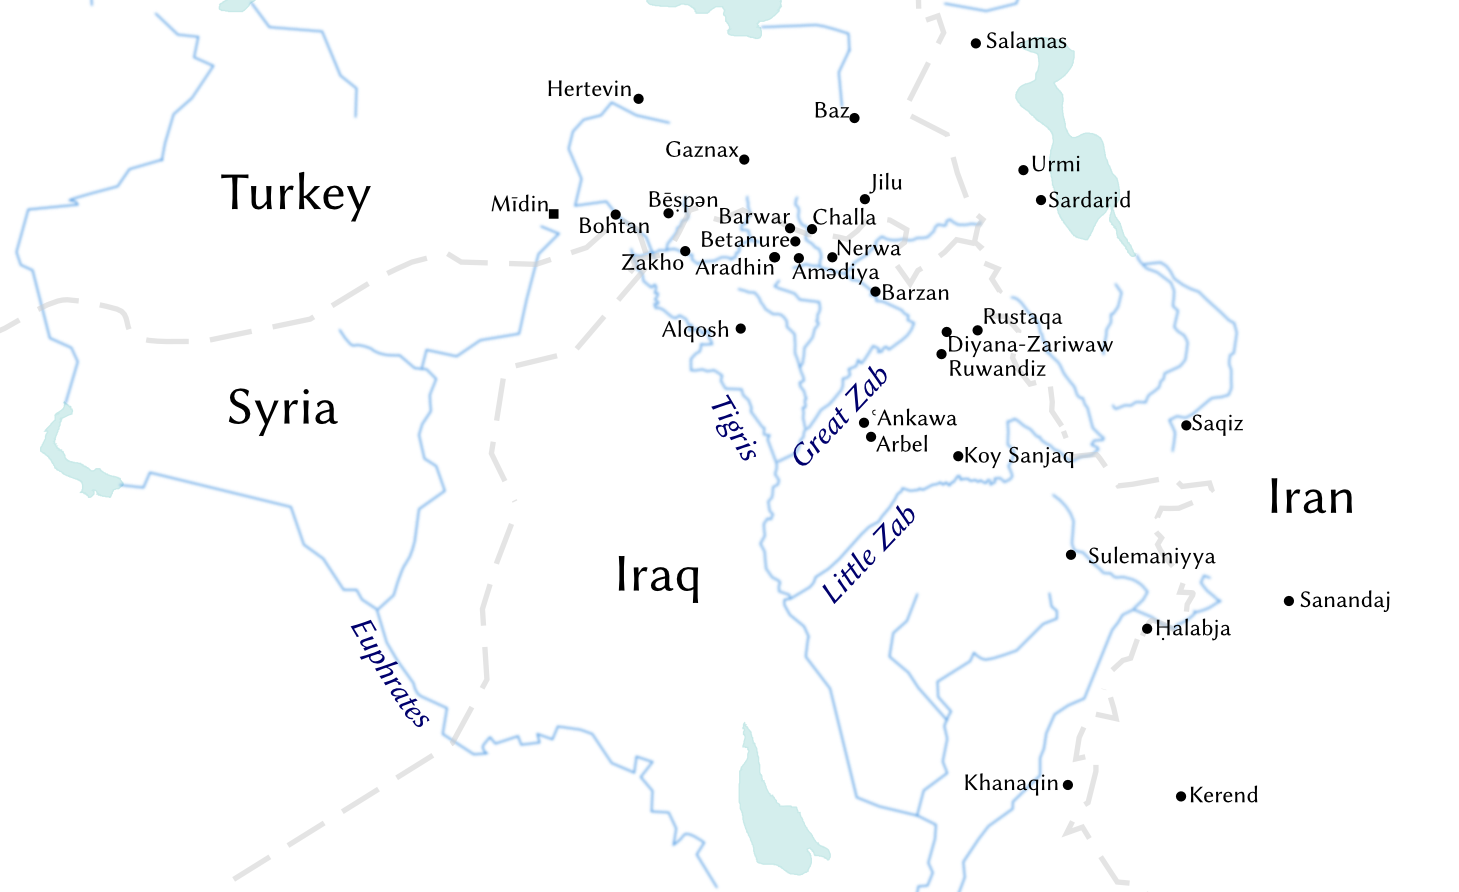
\includegraphics[width=\textwidth]{figures/NENAmap.png}
\caption{Approximate locations of NENA dialects (and one NWNA dialect: 
\Midn) at the beginning of the 20\th\ century.} \label{fg:map_nena}
\end{figure}


The amount of information gathered from the different sources varies considerably. Seven dialects (marked in \textbf{bold} in \ref{tb:dialects}) contributed each between 100 and 200 examples to the research database, together amounting  to two-thirds of the \ili{NENA} data-points in it. Not surprisingly, amongst these are the 4 dialects to which survey chapters are devoted. The remaining dialects contributed each between 8 to 60 examples each.  Data from the dialects of Khabur\il{NENA!Khabur dialects} \citep{TalayKhabur} were collected as well, but for methodological reasons are not treated in the book.


The data collected was registered in a Microsoft Access database. Accordingly, in this database all the various ACs found in the different \ili{NENA} dialects surveyed, as well as other  languages under investigation (mainly Kurdish and Syriac), were listed and linked to appropriate examples. The classification of the ACs in the database was done according to the principles outlined in \vref{ss:typology_here}. An example of the data-entry form is given in \vref{fg:ACform}. The database can be found online as part of \citet{GutmanThesis}.\footnote{In the electronic database the \prim and \secn fields are referred to as Nucleus and Attribute respectively.}

\begin{sidewaysfigure}[p]


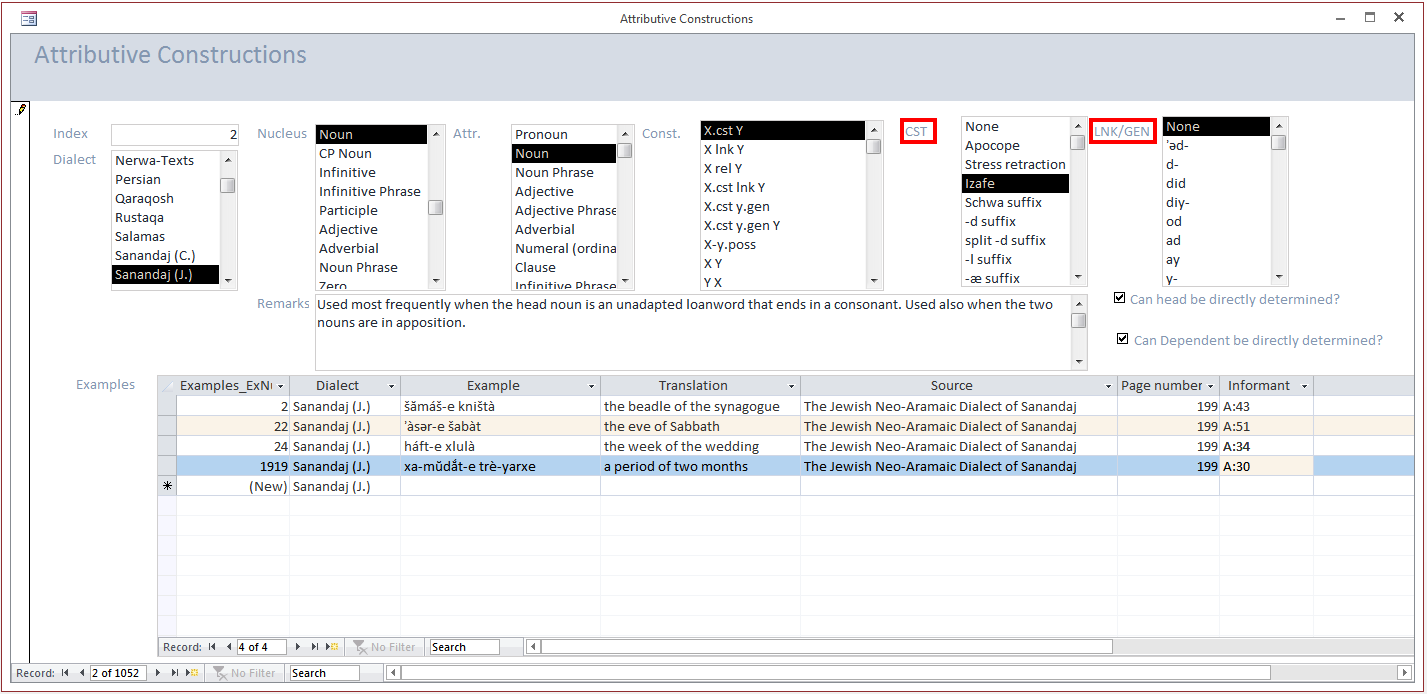
\includegraphics[width=\textheight]{figures/ACform.png}
\caption{Example of data entry in the accompanying database} \label{fg:ACform}
\end{sidewaysfigure}

 
While many of the consulted \ili{NENA} grammars have sections labelled \enquote{Annexation}, \enquote{Attributes} or the like, the concept of the \isi{attributive construction} as  defined in the current work is normally not described in any single section of the grammar, requiring collection of examples from numerous sections in a given grammar.\footnote{An exception is the grammar of \JZax, \citet{CohenZakho}.} The data assembly started with the collection of ACs headed by nouns modified by various attributes (nouns, adjectives, clauses etc.). Only subsequently were examples with other types of \prims (pronouns, adjectives, adverbials etc.)\ collected, yielding possibly a less systematic picture of these combinations. 

It should be noted that the listing of the different constructions is purely qualitative, as no quantitative data were gathered from the corpora. Thus, any remark regarding the usage frequency of a given construction is based on comments given in the consulted grammars.

The database design permits to query cross-dialectally the presence of a specific construction, with or without limitations to the parts-of-speech involved. This possibility was invaluable for conducting the comparative research, constituting the core of the current study (see chapters 10--11). 

\paragraph*{Format of examples} \label{ss:examples_format}
The \ili{NENA} examples given in this work are all taken from the database. While the database conserves the original transcription system of each source, in the book I have attempted to normalize the different transcriptions to a standard system, namely that of \citet{KhanBarwar, KhanSanandaj, KhanUrmi}.\footnote{Note that older publications of Khan, such as \citet{KhanArbel, KhanSulemaniyya} use a slightly different system. The main difference has to do with the transcription of a short \phonetic[ɪ]\~\phonetic[ə] vowel, which in later works is transcribed as \transc{ə}, while in earlier works it is transcribed as \transc{ĭ}.  Notwithstanding the question of transcription, it should be noted that not in all dialects is the difference between a tense \phonetic[i] and a lax \phonetic[ə] phonemic (see for instance the discussion of \Gaz phonemic inventory in \cite{GutmanGaznax}). Another change concerns the rendering in \ili{NENA} dialects of a fricative \phonetic[θ] consistently as \transc{θ} rather than \transc{ṯ}. Especially affected is the transcription system of \citet{YounansardaroudSardarid}, which I have simplified by removing the vocalic-timbre marks as well as most timbre superscripts \citep[cf.][20]{YounansardaroudSardarid}. The hard timbre which is marked by her as superscript \textsuperscript{h} is marked here with a ⁺ sign, in accordance with \citet{KhanUrmi}.}

 All examples have a title stating the language (or dialect) of the example as well as the categories of the members of the AC under discussion. Thus, a title of \textbf{Noun Phrase-Adjective} means that the example illustrates an AC with a noun phrase modified by an adjective, irrespective of the question of the ordering of the adjective and the noun phrase in the example itself, and the possibility of other (typically embedded) ACs appearing  in the example. The examples are glossed according to the Leipzig Glossing Rules \citep{LeipzigGlossingRules} with some additions (see list of glosses \vpageref{ap:glosses}). 
  
  Typically, the examples are cited using the source's page number where they are discussed (unless they are cited directly from a corpus). The original example number (if available) is given in parenthesis. If the author gives a reference to his own corpus (typically a letter+number combination), this is given in square brackets.
  
  The format of examples is illustrated \vpageref[below]{ex:example}.




\acex[Language]
{\Prim}{\Secn}{example}
{Example text}
{Glosses}
{Translation}
{}{(Source: page (example number) [Textual reference])}

